\documentclass{article}

\usepackage{listings}
\usepackage{color}
\usepackage{graphicx}
\graphicspath{ {images/} }

\definecolor{backcolor}{rgb}{0.95, 0.95, 0.95}

\lstdefinestyle{codestyle} {
    backgroundcolor=\color{backcolor}
}

\lstset{style=codestyle}

\title{
    Coding Standards\\
    \begin{large}
        \textit{Golf Course Mapper}
    \end{large}
}
\date{
    \begin{small}
        \today
    \end{small}
}
\author{
    Team Recursive Recursion
}

\begin{document}
    \pagenumbering{gobble}
    \maketitle
    \newpage
    \pagenumbering{arabic}
    
    \tableofcontents
    \newpage

    %===========================================================================

    \section{Introduction}
    \label{sec:intro}

    \subsection{Purpose}
    \label{sec:purp}

    This \textit{Coding Standards Document} is intended to be a guide on the
    policies, standards and practices that are followed when working on the
    \textit{Golf Course Mapper} project. The remainder of this section describes
    the different repositories used within the project and the remainder of this
    document then continues to describe the coding standards applied to each
    individual repository.

    \subsection{Repositories Structure}
    \label{sec:reps}

    There are four (4) repositories that are used for the project:
    \texttt{web-app}, \texttt{mobile-app}, \texttt{mapper-api} and
    \texttt{documentation}. A short description of the contents of each
    repository is listed below.

    \begin{itemize}
        \item \texttt{web-app}
            \subitem Contains web application subsystem used for mapping and
            managing golf courses. The web application is built using
            \textit{Angular 6}.
        \item \texttt{mobile-app}
            \subitem Contains the \textit{Android} app used for viewing golf
            courses. The mobile app is built using native Java code.
        \item \texttt{mapper-api}
            \subitem Contains the \textit{Entity Framework Core} API used to
            manage and provide access to the database. The database used is
            \textit{PostGIS}, an extention of \textit{PostgreSQL}.
        \item \texttt{documentation}
            \subitem Contains all documentation relating to the project,
            including this file. Documents are written in \LaTeX. The repository
            also contains all additional images and published PDF versions of
            the documents.
    \end{itemize}

    \newpage

    %===========================================================================

    \section{Global Standards}
    \label{sec:global}

    The following standards are applied to all files across all repositories,
    with the exclusion of automatically generated files.

    \subsection{File Format}
    \label{sec:file-format}

    \begin{itemize}
        \item Files are encoded using the \textbf{UTF-8} character set.
        \item Lines should not be longer than \textbf{80 columns}.
        \item \textbf{Soft tabs} expanded to \textbf{4 spaces} should be used.
        \item Each level of indentation uses \textbf{1 tab}.
        \item Line continuation indentation uses \textbf{2 tabs}.
        \item Every file contains a \textbf{file header}.
    \end{itemize}

    \subsection{File Header Layout}
    \label{sec:file-headers}

    Headers are always on the first line of a file and are placed in comments.
    The following information must always be present where applicable:

    \begin{itemize}
        \item Name of the file
        \item Original author of the file
        \item Name of the class(es) contained within the file
        \item Short description of the file
    \end{itemize}

    The file header layout is illustrated below. The \texttt{(start)} and
    \texttt{(end)} tags indicate the block-comment start and end symbols.
    As these are language specific, they are described in the sections
    dealing with per-language standards.

    \begin{lstlisting}
(start)
    Filename: File.ext
    Author  : John Doe
    Class   : SampleClass

        The SampleClass contains many different sample
        methods.
(end)
    \end{lstlisting}

    \newpage

    %===========================================================================

    \section{Web App Standards}
    \label{sec:web-app}

    This section describes the coding standards applied to the \texttt{web-app}
    repository. %The system design of the subsystem is illustrated in Section
    %\ref{sec:wa-design} and
    The file structure of the repository is explained in
    Section \ref{sec:wa-struc}. The web application makes use of TypeScript,
    HTML and CSS. The standards for these languages are described in Sections
    \ref{sec:typescript} and \ref{sec:html-css}.

    %\subsection{System Design}
    %\label{sec:wa-design}

    %UML class diagram coming soon\ldots

    \subsection{File Structure}
    \label{sec:wa-struc}

    The repository contains a \texttt{WebApplication/} folder at the root which
    contains the source files of the subsystem. This folder was created through
    the Angular CLI, and are therefore organized according to the standard
    Angular layout.

    The most important folder is the \texttt{src/} folder, which contains the
    following notable locations:

    \begin{itemize}
        \item \texttt{app/}
            \subitem This folder contains all of the source code of the web
            application. The most important files here are
            \texttt{app.component.ts} and \texttt{app.module.ts} which describe
            the root Angular components.
        \item \texttt{app/components/}
            \subitem This folder contains different subfolders. Each subfolder
            represents one of the components as represented in Section
            \ref{sec:wa-design}. Each subfolder contains the \texttt{.html} and
            \texttt{.ts} files associated with each component.
        \item \texttt{app/interfaces/}
            \subitem This folder contains the \texttt{.ts} files that describe
            the enums and interfaces used in the web app.
        \item \texttt{app/services/}
            \subitem This folder contains different subfolders. Each subfolder
            represents one of the services as represented in Section
            \ref{sec:wa-design}. Each subfolder contains the \texttt{.ts} files
            associated with each service.
        \item \texttt{assets/}
            \subitem This folder contains all the assets such as background
            images and icons used within the web app.
    \end{itemize}

    \subsection{Typescript Standards}
    \label{sec:typescript}

    \subsubsection{Naming Conventions}
    \label{sec:typescript-nc}

    \begin{itemize}
        \item \textbf{Variables} are named using camel casing. Descriptive names
                should be used with the exception of counters in loops.
        \item \textbf{Classes} start with a \textit{capital} letter and use
                camel casing.
        \item \textbf{Components} must have the word \texttt{Component} as the
                last word in the class name. Similarly, \textbf{Services} must
                have \texttt{Service} as the last word.
        \item \textbf{Functions} are also named similar to regular variables and
                should be descriptive.
    \end{itemize}

    \begin{lstlisting}
export class SampleComponent {

    sampleVariable : string;

    public myFunction() : void {
        ...
    }
}
    \end{lstlisting}

    \subsubsection{Style}
    \label{sec:typescript-st}

    \paragraph{}
    \textbf{Braces} will be styled in the following manner:
    \begin{itemize}
        \item Opening braces are placed on the same line as the header.
        \item Closing braces are placed on a separate line at the same
                indentation level as the header.
        \item Else clauses are placed on the same line as the closing brace.
        \item While clauses of a do-while are placed on the same line as the
                closing brace.
        \item Braces are never left out for one-line loops or conditions.
    \end{itemize}

    \begin{lstlisting}
if (condition) {
    statement;
} else {
    statement;
}

while (condition) {
    statement;
}

do {
    statement;
} while (condition);
    \end{lstlisting}

    \textbf{Continuation lines} should end on the operator as to indicate that
    the line is not complete and has a continuation.

    \begin{lstlisting}
var result = example + of + (a * very) / 
        long - equation;
    \end{lstlisting}

    \subsubsection{Comments}
    \label{sec:typescript-com}

    \paragraph{}
    \textbf{File headers} are structured according to section
    \ref{sec:file-headers} and are styled in the following way:

    \begin{lstlisting}
/***
 * Filename: sample.component.ts
 * Author  : John Doe
 * Class   : SampleComponent
 *
 *     The SampleComponent contains many different sample
 *     methods.
 ***/
    \end{lstlisting}

    \textbf{Function headers} are provided for every function and take the
    following form (the description can be omitted in the case of simple
    functions, such as mutators \& accessors).

    \begin{lstlisting}
/***
 * function(ParType1, ParType2) : ReturnType
 *
 *     Description of the function.
 ***/
function(p1 : ParType1, p2 : ParType2) : ReturnType {
    ...
}
    \end{lstlisting}

    \textbf{Inline comments} should be kept to a minimum, since code should be
    self-documenting. Only use inline comments in the case of code that may be
    difficult to understand.

    \subsection{HTML \& CSS Standards}
    \label{sec:html-css}

    \subsubsection{Style}
    \label{sec:ls-html-st}

    \paragraph{}
    \textbf{CSS} files should be styled in the following way:

    \begin{lstlisting}
selectors {
    some-attribute: style;
    another-attribute: style;
}

more {
    some-attribute: style;
}
    \end{lstlisting}

    \textbf{HTML} files should be styled according to the following rules:

    \begin{itemize}
        \item Opening and closing tags of \textbf{block} elements should be kept
            on their own lines, with the content indented.
        \item Opening and closing tags of \textbf{inline} elements should be
            kept on the same line, with the content between the tags.
    \end{itemize}

    \begin{lstlisting}[language=html]
<div>
    <p>
        Here is some <span class="red">red</span> text!
    </p>
</div>
    \end{lstlisting}

    \subsubsection{Comments}
    \label{sec:ls-html-com}

    \paragraph{}
    \textbf{File headers} are structured according to section
    \ref{sec:file-headers} and are styled for CSS and HTML, respectively, in the
    following ways:

    \begin{lstlisting}
/***
 * Filename: style.css
 * Author  : John Doe
 *
 *     The styling for some example page is contained
 *     here and applies a material style.
 ***/
    \end{lstlisting}

    \begin{lstlisting}
<!--
    Filename: page.html
    Author  : John Doe
    
        The page displays some content.
-->
    \end{lstlisting}

    \newpage
    
    %===========================================================================

    \section{Mobile App Standards}
    \label{sec:mobile-app}

    This section describes the coding standards applied to the
    \texttt{mobile-app} repository. The system design of the subsystem is
    illustrated in Section \ref{sec:ma-design} and the file structure of the
    repository is explained in Section \ref{sec:ma-struc}. The mobile
    application makes use of Java. The standards for the Java language are
    described in Section \ref{sec:java}.

    \subsection{System Design}
    \label{sec:ma-design}

    \begin{figure}[h!]
        \centering
        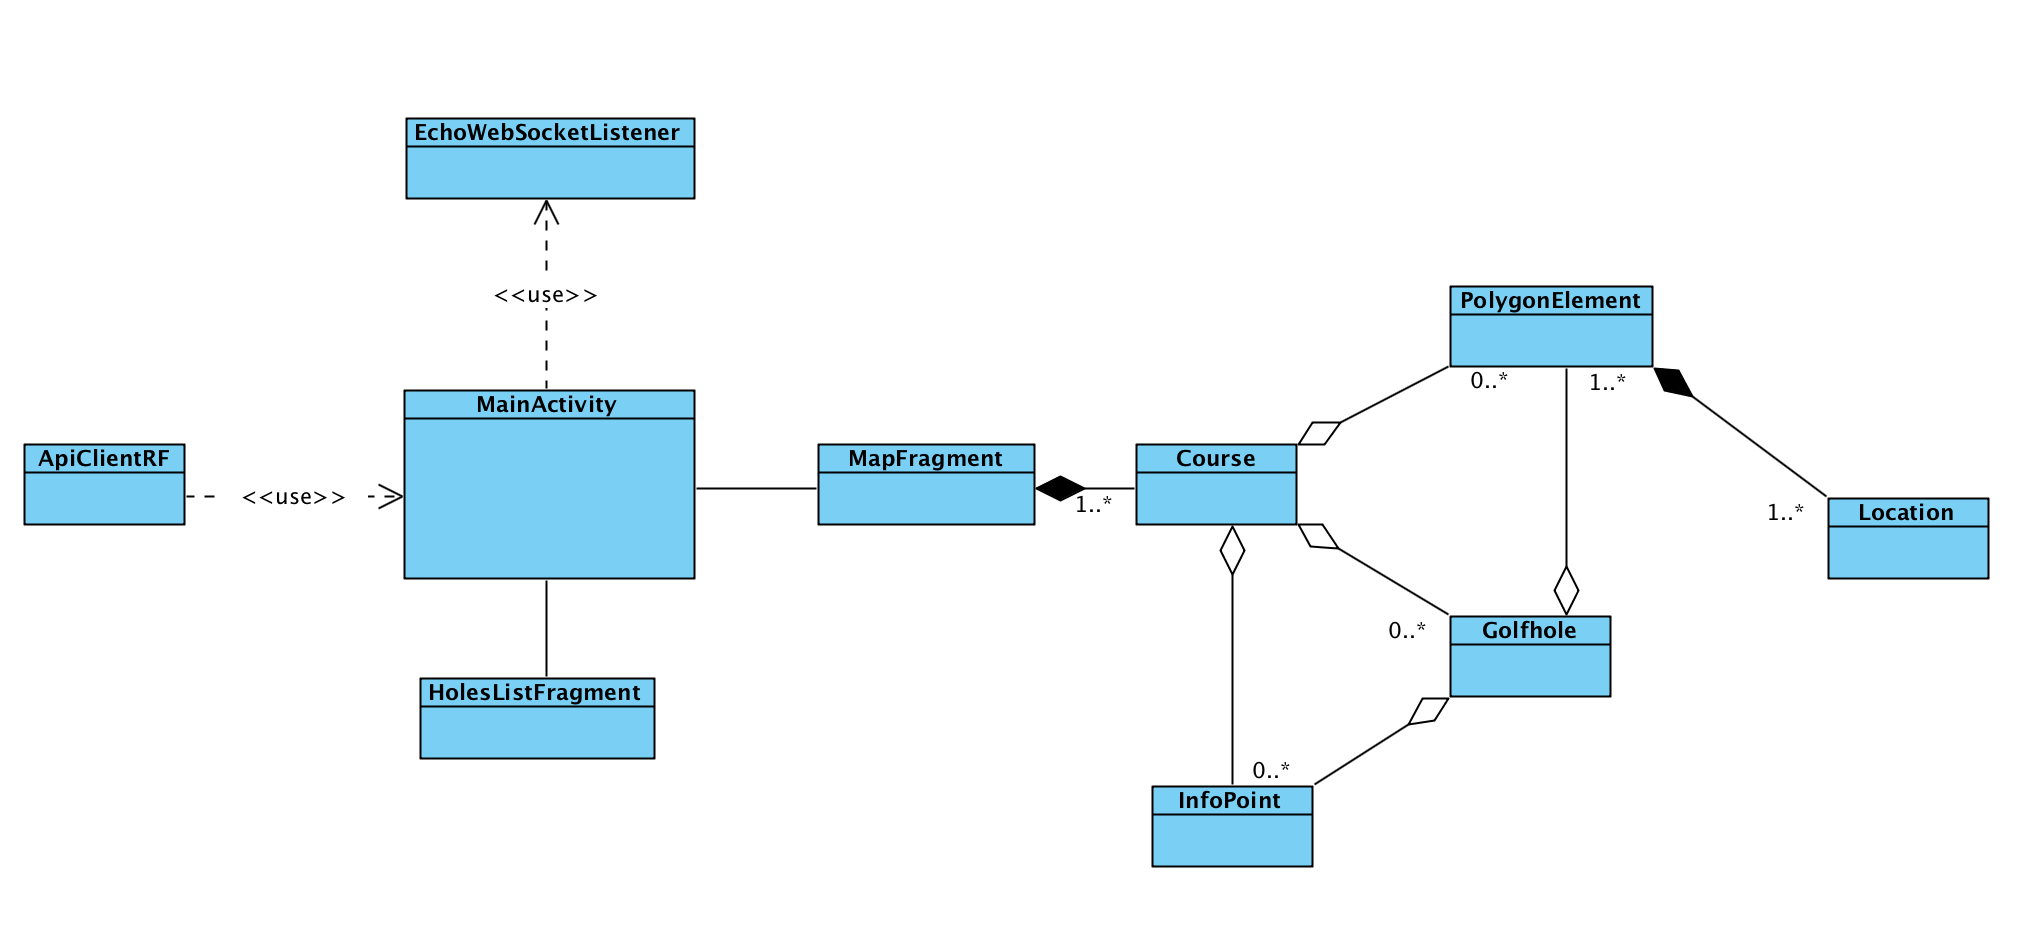
\includegraphics[scale=0.4]{MobileClassDiagram}
        \caption{UML Class Diagram of the Mobile Application}
        \label{fig:mobuml}
    \end{figure}

    \subsection{File Structure}
    \label{sec:ma-struc}

    The root of the repository contains the \textit{Android Studio} project
    folder and is therefore organized according to the standard \textit{Android
    Studio} layout.

    \subsection{Java Standards}
    \label{sec:java}

    \subsubsection{Naming Conventions}
    \label{sec:java-nc}

    \begin{itemize}
        \item \textbf{Variables} are named using camel casing. Descriptive names
                should be used with the exception of counters in loops.
        \item \textbf{Member variables} are named similarly to regular variables
                with the addition of an \textit{underscore} prefix.
        \item \textbf{Classes} start with a \textit{capital} letter and use
                camel casing.
        \item \textbf{Functions} are also named similar to regular variables and
                should be descriptive.
    \end{itemize}

    \begin{lstlisting}[language=java]
class SampleClass {

    int _someMember;

    public void myFunction() {
        int someInteger;
    }
}
    \end{lstlisting}

    \subsubsection{Style}
    \label{sec:java-st}

    \paragraph{}
    \textbf{Braces} will be styled in the following manner:
    \begin{itemize}
        \item Opening braces are placed on the same line as the header.
        \item Closing braces are placed on a separate line at the same
                indentation level as the header.
        \item Else clauses are placed on the same line as the closing brace.
        \item While clauses of a do-while are placed on the same line as the
                closing brace.
        \item Braces are never left out for one-line loops or conditions.
    \end{itemize}

    \begin{lstlisting}[language=Java]
if (condition) {
    statement;
} else {
    statement;
}

while (condition) {
    statement;
}

do {
    statement;
} while (condition);
    \end{lstlisting}

    \textbf{Continuation lines} should end on the operator as to indicate that
    the line is not complete and has a continuation.

    \begin{lstlisting}[language=Java]
double result = example + of + (a * very) / 
        long - equation;
    \end{lstlisting}

    \subsubsection{Comments}
    \label{sec:java-com}

    \paragraph{}
    \textbf{File headers} are structured according to section
    \ref{sec:file-headers} and are styled in the following way:

    \begin{lstlisting}[language=Java]
/***
 * Filename: SampleClass.java
 * Author  : John Doe
 * Class   : SampleClass
 *
 *     The SampleClass contains many different sample
 *     methods.
 ***/
    \end{lstlisting}

    \textbf{Function headers} are provided for every function and take the
    following form (the description can be omitted in the case of simple
    functions, such as mutators \& accessors).

    \begin{lstlisting}[language=Java]
/***
 * function(ParType1, ParType2) : ReturnType
 *
 *     Description of the function.
 ***/
ReturnType function(ParType1 p1, ParType2 p2) {
    ...
}
    \end{lstlisting}

    \textbf{Inline comments} should be kept to a minimum, since code should be
    self-documenting. Only use inline comments in the case of code that may be
    difficult to understand.

    \newpage

    %===========================================================================

    \section{Mapper API Standards}
    \label{sec:mapper-api}

    This section describes the coding standards applied to the
    \texttt{mapper-api} repository.% The system design of the subsystem is
    %illustrated in Section \ref{sec:api-design} and 
    The file structure of the
    repository is explained in Section \ref{sec:api-struc}. The API makes use of
    C\#. The standards for the C\# language are described in Section
    \ref{sec:cs}.

    %\subsection{System Design}
    %\label{sec:api-design}

    %UML class diagram coming soon\ldots

    \subsection{File Structure}
    \label{sec:api-struc}

    The root of the repository contains the \texttt{Test} and \texttt{MapperApi}
    folders. The \texttt{Test} folder contains all the Unit Test files as
    described further in the \textit{Testing Policy Document}. The
    \texttt{MapperApi} folder is the \textit{Entity Framework Core} project
    folder and is therefore organized according to the standard \textit{Entity
    Framework Core} file layout.

    \subsection{C\# Standards}
    \label{sec:cs}

    \subsubsection{Naming Conventions}
    \label{sec:cs-nc}

    \begin{itemize}
        \item \textbf{Variables} are named using camel casing. Descriptive names
                should be used with the exception of counters in loops.
        \item \textbf{Member variables} are named similarly to regular variables
                with the addition of an \textit{underscore} prefix.
        \item \textbf{Classes} start with a \textit{capital} letter and use
                camel casing.
        \item \textbf{Functions} are also named similar to regular variables and
                should be descriptive.
    \end{itemize}

    \begin{lstlisting}[language=java]
class SampleClass {
    int _someMember;

    public void myFunction() {
        int someInteger;
    }
}
    \end{lstlisting}

    \subsubsection{Style}
    \label{sec:cs-st}

    \paragraph{}
    \textbf{Braces} will be styled in the following manner:
    \begin{itemize}
        \item Opening braces are placed on the same line as the header.
        \item Closing braces are placed on a separate line at the same
                indentation level as the header.
        \item Else clauses are placed on the same line as the closing brace.
        \item While clauses of a do-while are placed on the same line as the
                closing brace.
        \item Braces are never left out for one-line loops or conditions.
    \end{itemize}

    \begin{lstlisting}[language=Java]
if (condition) {
    statement;
} else {
    statement;
}

while (condition) {
    statement;
}

do {
    statement;
} while (condition);
    \end{lstlisting}

    \textbf{Continuation lines} should end on the operator as to indicate that
    the line is not complete and has a continuation.

    \begin{lstlisting}[language=Java]
double result = example + of + (a * very) / 
        long - equation;
    \end{lstlisting}

    \subsubsection{Comments}
    \label{sec:cs-com}

    \paragraph{}
    \textbf{File headers} are structured according to section
    \ref{sec:file-headers} and are styled in the following way:

    \begin{lstlisting}[language=Java]
/***
 * Filename: SampleClass.cs
 * Author  : John Doe
 * Class   : SampleClass
 *
 *     The SampleClass contains many different sample
 *     methods.
 ***/
    \end{lstlisting}

    \textbf{Function headers} are provided for every function and take the
    following form (the description can be omitted in the case of simple
    functions, such as mutators \& accessors).

    \begin{lstlisting}[language=Java]
/***
 * function(ParType1, ParType2) : ReturnType
 *
 *     Description of the function.
 ***/
ReturnType function(ParType1 p1, ParType2 p2) {
    ...
}
    \end{lstlisting}

    \textbf{Inline comments} should be kept to a minimum, since code should be
    self-documenting. Only use inline comments in the case of code that may be
    difficult to understand.

    \newpage

    %===========================================================================

    \section{Documentation Standards}
    \label{sec:documentation}

    This section describes the standards of the \texttt{documentation}
    repository. As there are no strict standards for the layout of the \LaTeX
    files, only the file structure of the repository is described in Section
    \ref{sec:doc-struc}.

    \subsection{File Structure}
    \label{sec:doc-struc}

    The repository contains a folder for each of the four documents, namely
    \texttt{coding-standards/}, \texttt{requirements/}, \texttt{testing-policy/}
    and \texttt{user-manual/}. Each folder contains the \texttt{.tex} source
    file of the document as well as any additional files required for the
    document, such as images.

    The \texttt{publish} folder contains publish-ready versions of the documents
    in \textit{PDF} format.

    Finaly, the \texttt{other} folder contains extra documents that do not form
    part of the main documents, but are used elsewhere such as on the landing
    page.

    \newpage

    %===========================================================================

    \section{Code Review}
    \label{sec:review}

    This section describes how and when code is reviewed. It further describes
    who is responsible for reviewing code.

    \subsection{Review Process}
    \label{sec:review-proc}

    Before a pull request to the \texttt{master-dev} branch is accepted, the
    reviewer responsible for that repository must review the code. Code is
    only reviewed before mergin to \texttt{master-dev}, as that will ensure
    that \texttt{master} is also always up to standard.

    The code reviewer will review the code through inspection by looking at the
    changes proposed in the pull request. If the code complies to the
    repository's standards as described in this document and the build succeeds,
    the pull request is accepted.

    If the code does not comply to the repository's standards, the person
    responsible for the code is notified and must ammend the pull request to
    change the code. Once the code complies to the standards, the pull
    request is then accepted.

    \subsection{Responsible Party}
    \label{sec:review-party}

    A single person is assigned to a specific repository during the weekly scrum
    meetings. The person is assigned for a period of two weeks after which a new
    person (or possibly the same person again) is assigned to the repository.
    This person is solely responsible for performing the code review process (as
    described in Section \ref{sec:review-proc}) on the assigned repository.

\end{document}
